\begin{XeClass}{Syncable}
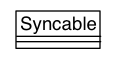
\includegraphics[width=10cm]{cdig/Syncable.png}
     
 这个接口声明了对Client的buffer进行flush的操作,此接口主要被
 BufferedIOStream实现。
 
 此接口的两个主要方法hflush、hsync的设计目的不同,hsync的目的是在执行
 完之后,保证数据
 会写在磁盘上,而hflush只会保证对数据源的新Client会读到刚flush的数据。
 
 在现在分析的HDFS版本中,这个接口的hflush和hsync方法一样,hsync会调用
 hflush。再后来2.x版本中,这两个方法将会有不同的实现。

\end{XeClass}
